\documentclass[border=2pt]{standalone}
\usepackage{tikz}
\begin{document}
\setbox0=\hbox{$e^{-x/2}\sin x$}
\typeout{TIKZKIT-SCRIPTED-WIDTH:\the\wd0}
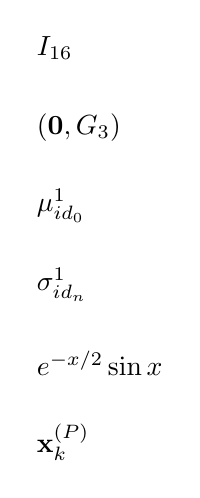
\begin{tikzpicture}
  \node[anchor=west] at (0,0) {$I_{16}$};
  \node[anchor=west] at (0,-1) {$({\bf 0},G_3)$};
  \node[anchor=west] at (0,-2) {$\mu_{id_0}^1$};
  \node[anchor=west] at (0,-3) {$\sigma_{id_n}^1$};
  \node[anchor=west] at (0,-4) {$e^{-x/2}\sin x$};
  \node[anchor=west] at (0,-5) {$\mathbf{x}_k^{(P)}$};
\end{tikzpicture}
\end{document}
